\documentclass{beamer}

% Beamer style
\usetheme{CambridgeUS}
\usecolortheme[rgb={0.65,0.15,0.25}]{structure}
\beamertemplatenavigationsymbolsempty

% Packages
\usepackage[latin1]{inputenc}
\usepackage{color}
\usepackage{amsmath, amsfonts, amssymb}
\usepackage{epsfig}
\usepackage{graphicx}

% Commands
\definecolor{darkred}{rgb}{0.65,0.15,0.25}
\definecolor{darkgreen}{rgb}{0,0.4,0}
%\newcommand{\emphase}[1]{\textcolor{darkred}{#1}}
\newcommand{\emphase}[1]{{#1}}
\newcommand{\paragraph}[1]{\textcolor{darkred}{#1}}
\newcommand{\refer}[1]{\textcolor{gray}{\cite{#1}}}
\newcommand{\Refer}[1]{\textcolor{gray}{#1}}
\newcommand{\newblock}{}
\newcommand{\ra}{$\emphase{\rightarrow}$}

% Names
\newcommand{\chr}{}
\newcommand{\figres}{}
\newcommand{\comment}{}

% Plot examples
%#2 = \figdir, #3 = \figname or \resname
\newcommand{\plotex}[4]{
  \begin{array}{cc}
    \begin{tabular}{p{.45\textwidth}}
      {#1}
    \end{tabular}
    &
    \hspace{-1cm}
    \begin{tabular}{p{.5\textwidth}}
      \includegraphics[width=.5\textwidth, height=.45\textheight]{#2/#3-LRR}
    \end{tabular} \\
    \hspace{-0.5cm}
    \begin{tabular}{p{.5\textwidth}}
      \includegraphics[width=.5\textwidth, height=.45\textheight]{#2/#3-BAF}
    \end{tabular}
    &
    \hspace{-1cm}
    \begin{tabular}{p{.5\textwidth}}
      \includegraphics[width=.5\textwidth, height=.45\textheight]{#2/#3-AB}
    \end{tabular} \\    
  \end{tabular}
}

%====================================================================
\title[Identifiability in HMM]{Identifiability in Hidden Markov Models \\ Applications to Loss of Heterozygocity (LOH)}

\author[S. Robin]{S. Robin}

\institute[AgroParisTech / INRA]{
  \bigskip
 \begin{tabular}{ccccc}
    
\includegraphics[width=.2\textwidth]{../Figures/LogoINRA-Couleur} & 
    \hspace{.02\textwidth} &
    
\includegraphics[width=.3\textwidth]{../Figures/logagroptechsolo} & 
    \hspace{.02\textwidth} &
    
\includegraphics[width=.2\textwidth]{../Figures/logo-ssb} \\ 
  \end{tabular} \\
  \bigskip
  {\normalsize
    \begin{tabular}{rll}
    Joint work with & E. Gassiat, & A. Cleynen, \\
    and & C. B�rard, & S. Volant \\
    \end{tabular}
    }
  }

  \date[WGMBC]{WGMBC, Bologna, July 2013}

%====================================================================

%====================================================================
%====================================================================
\begin{document}
%====================================================================
%====================================================================

%====================================================================
\frame{\titlepage
  }
  
%====================================================================
\section*{Identifiability in mixture models}
\frame{\frametitle{Identifiability in mixture models}
  }
  
%====================================================================
\frame{\frametitle{Identifiability in mixture models: An issue}

  \begin{tabular}{cc}
    \begin{tabular}{p{0.4\textwidth}}
	 \onslide+<1->{
	   \paragraph{Model-based clustering:} 
	 }
	 \onslide+<2->{
	 \begin{eqnarray*}	
	  \{Z_t\} \text{ iid} & \sim & {\mathcal M}(1; \pi), \\
	  (X_t | S_t = k) & \sim & \phi_k 
	 \end{eqnarray*} \\
	 }
	 \onslide+<3->{%\bigskip
	 Constraints on the $\phi_k$ are needed to insure identifiability
	 }
    \end{tabular}
    &
    \hspace{-0.05\textwidth}
    \begin{tabular}{p{0.5\textwidth}}
	 \begin{overprint}   
	 \onslide<1>    
	 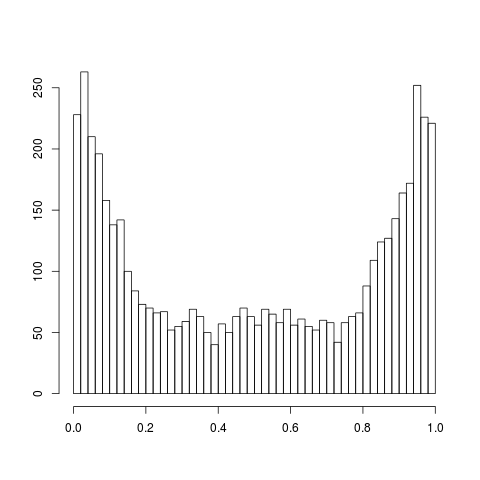
\includegraphics[height=.7\textheight]{../Figures/FigIndetif-BetaMixt0}
	 \onslide<2>
	 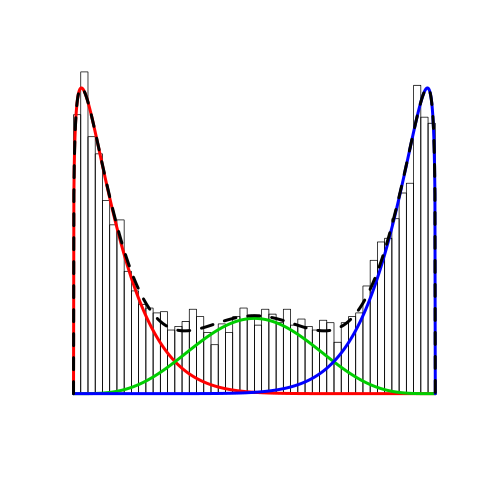
\includegraphics[height=.7\textheight]{../Figures/FigIndetif-BetaMixt1}
	 \onslide<3>
	 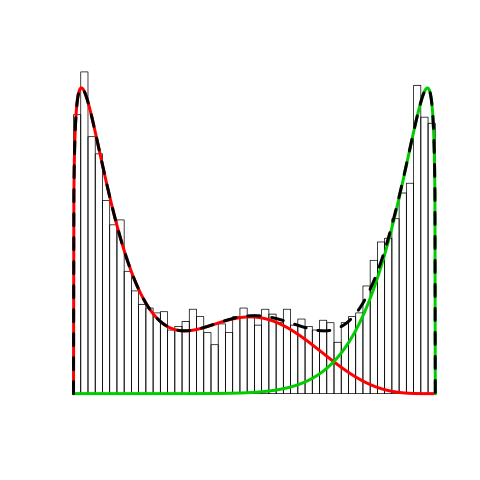
\includegraphics[height=.7\textheight]{../Figures/FigIndetif-BetaMixt2}
	 \onslide<4>
	 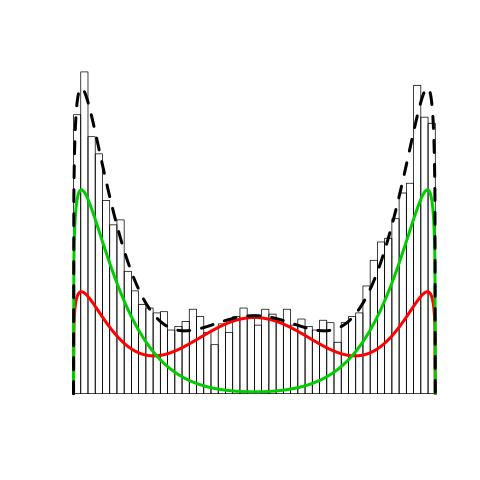
\includegraphics[height=.7\textheight]{../Figures/FigIndetif-BetaMixt3}
	 \end{overprint}   
    \end{tabular}
  \end{tabular}
  }

%====================================================================
\frame{\frametitle{Outline}
  \setcounter{tocdepth}{1}
  \tableofcontents
  }
  
%====================================================================
\section{Identifiability in hidden Markov models}
\frame{\frametitle{Identifiability in hidden Markov models}
  }
  
%====================================================================
\subsection{Identifiability}
\frame{\frametitle{Identifiability}
  
  \paragraph{Definition:} A model $P_\theta$ is identifiable iff two different parameters yield two different likelihood functions:
  $$
  \theta \neq \theta' \qquad \Rightarrow \qquad P_\theta(\cdot) \neq P_{\theta'}(\cdot).
  $$
  
  \bigskip
  Identifiability is a desirable property for both 
  \begin{itemize} 
  \item theoretical reasons, e.g. consistency of MLEs and
  \item practical reasons, e.g. interpretation of the results.
  \end{itemize}

  \bigskip \bigskip
  Non-identifiability issues often arise in latent variables or state-space models.
  }
  
%====================================================================
\frame{\frametitle{State space models}

  \paragraph{Finite mixture models.} Flexible emission distributions do not meet identifiability (besides label swapping) in general.
  \begin{itemize}
   \item mixture \refer{BRC10};
   \item fully non-parametric.
  \end{itemize}
  
  \bigskip
  \paragraph{Some exceptions are known,} e.g. non-parametric emission distributions:
   \begin{itemize}
   \item with shape constraints \refer{BMV06,GaR13}, 
   \item in presence of known components \refer{BDV06,RBD07},
   \item when multivariate with independent coordinates \refer{AMR09};
  \end{itemize}
  
  \bigskip
  \paragraph{Hidden Markov models.} Some dependency in the hidden layer may yield identifiability, e.g.
  finite hidden Markov models with finite discrete emission distributions \refer{Pet69}.
  }

%====================================================================
\frame{\frametitle{A previous result}
  
  \paragraph{Allmann \& al. (2009, \refer{AMR09}), Theorem 9:} The mixture with product emissions
  $$
  \sum_{k = 1}^K \pi_k \Phi_k(\cdot), \qquad \Phi_k(\cdot) = \prod_{j=1}^p \phi_{kj}(\cdot)
  $$
  is identifiable (up to label swapping) as soon as:
  \begin{enumerate}
  \item the distributions $\{\phi_{kj}(\cdot)\}_k$ are linearly independent;
  \item $p \geq 3$.
  \end{enumerate}

  \bigskip \bigskip
  \paragraph{Historical remark.}
  The proof relies on a result of Kruskall (1977, \refer{Kru77}) for 3-way contingency tables.
 }

%====================================================================
\subsection{Hidden Markov models}
\frame{\frametitle{Hidden Markov models}

  \paragraph{Model.}  
  \begin{itemize}
   \item $S = (S_t)_t$: unobserved ergodic Markov chain over $\{1, \dots K\}$ with transition matrix $\pi$;
   \item $Y = (Y_t)_t$: observed data, independent conditional on $S$ with emission distribution
   $$
   (Y_t | S_t = k) \sim \phi_k.
   $$
  \end{itemize}
 
  \bigskip \bigskip
  \begin{theorem}[Gassiat \& al, 2013 \refer{GCR13}]
  The model is identifiable provided that  
  \begin{enumerate}[($a$)]
   \item the emission distributions $(\phi_k)_k$ are linearly independent and
   \item the transition matrix $\pi$ has rank $K$.
  \end{enumerate}
  \end{theorem}
  }

%====================================================================
\frame{\frametitle{Identifiability in HMM}

  \paragraph{Sketch of proof.}  $(Y_{t-1}, Y_t, Y_{t+1})$ are independent, conditional on $(S_{t-1}, S_t, S_{t+1})$, so the joint distribution of $(Y_{t-1}, Y_t, Y_{t+1})$ is a mixture\footnote{$\nu =$ stationary distribution of $\pi$.}
  \begin{eqnarray*}
  (Y_{t-1}, Y_t, Y_{t+1}) & \sim & \sum_{i, j, k} \nu_i \; \pi_{ij} \; \pi_{jk} \; \phi_i(y_{t-1}) \; \phi_j(y_t) \; \phi_k(y_{t+1})  \\
  & = & \sum_{i, j, k} \Pi_{ijk} \Phi_{ijk}(y_{t-1}, y_t, y_{t+1}),
  \end{eqnarray*}
  \begin{itemize}
  \item with proportions $\Pi_{ijk} = \nu_i \; \pi_{ij} \; \pi_{jk}$ 
  \item and product emission distributions $\Phi_{ijk}(u, v, w) = \phi_{i}(u) \phi_{j}(v) \phi_{k}(w)$
  \end{itemize}
  so Theorem 9 of \refer{AMR09} applies.
  }

%====================================================================
\frame{\frametitle{Some consequences (and comments)}

  \paragraph{Modeling.}
  Under mild conditions, HMM non-parametric distributions or mixtures emissions make sense.
  
  \bigskip \bigskip
  \paragraph{Inference.} The result suggest the use of the pseudo-(log-)likelihood
  $$
  \sum_{t} \log P_\theta(Y_{t-1}, Y_t, Y_{t+1})
  $$
  as an alternative to EM.
  
  \bigskip \bigskip
  \paragraph{Real life.} We still have few experience on the way non-parametric HMMs behave in practice.
  $$
  \text{\ra \quad A lot of open problems remain.}
  $$
  }


%====================================================================
\section{A classification problem in genomics}
\frame{\frametitle{A classification problem in genomics}
  }

%====================================================================
\subsection{Genotyping using SNP}
\frame{\frametitle{Genotyping using SNP}

  \paragraph{SNP =} Single Nucleotide Polymorphism:
  $$
  \begin{tabular}{cc}
   allele A: & {\tt a g g c }\textcolor{red}{\tt g }{\tt c t a g} \\
   allele B: & {\tt a g g c }\textcolor{red}{\tt a }{\tt c t a g} 
  \end{tabular}
  $$

  \bigskip
  \paragraph{Applications:} \\
  Association studies, population genetics, forensics... more to come.

  \bigskip \bigskip \bigskip
  \paragraph{SNP array.} $n \simeq 10^5 - 10^6$ loci along the human genome
  \begin{itemize}
   \item $A_t =$ signal associated with allele A at locus $t$
   \item $B_t =$ signal associated with allele B at locus $t$
  \end{itemize}
  \ra \quad Observed data: $Y_t = (A_t, B_t).$

  }

%====================================================================
\frame{\frametitle{Various use of SNP arrays (and classification problems)}

\newcommand{\figPopova}{/home/robin/RECHERCHE/RUPTURES/LOH/Data/Popova}
\renewcommand{\chr}{11}


  %\vspace{-0.5cm}
  \begin{tabular}{cc}
    \hspace{-0.5cm}
    \begin{tabular}{p{.4\textwidth}}
    \onslide+<1->{\paragraph{SNP calling:} Classify into one genotype
      $$
      Z_t  \in \{\text{AA}, \text{AB}, \text{BB}\}.
      $$}
    \onslide<2->{\hspace{-.015\textwidth}\paragraph{CNV = Copy Number Variation:} Normal cells possess 2 copy of each locus: \\
      $$
      A_t + B_t \propto 2.
      $$}
    \onslide<3->{\hspace{-.015\textwidth}\paragraph{LOH = Loss Of Heterozygocity:} Normal cells can be  heterozygous at any locus:
      $$
      BAF_t \in \{0, 1/2, 1\}.
      $$}
    \end{tabular}
    &
    \hspace{-.05\textwidth}
    \begin{overprint}
      \onslide<1>
      \begin{tabular}{c}
	$BAF_t = B_t/(A_t+B_t)$ \\
	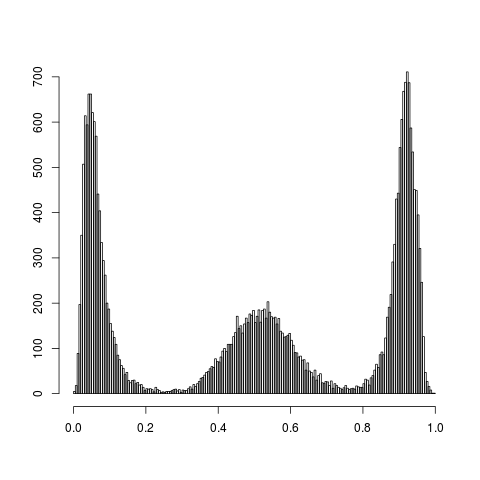
\includegraphics[width=.5\textwidth, clip=]{../Figures/NA06991-Chr6BAFraw}\\
	Data from \refer{SLV08}, chromosome 6.
      \end{tabular}
      \onslide<2>
      \begin{tabular}{c}
	$A_t+B_t = f(\text{locus } t)$\\
	\includegraphics[width=.5\textwidth, clip=]{\figPopova/R_BLC_B1_T45-Chr\chr-LRR} \\
	Data from \refer{PMS09}, chromosome \chr.
      \end{tabular}
      \onslide<3>
      \begin{tabular}{c}
	$BAF_t = f(\text{locus } t)$ \\
	\includegraphics[width=.5\textwidth, clip=]{\figPopova/R_BLC_B1_T45-Chr\chr-BAF} \\
	Data from \refer{PMS09}, chromosome \chr.
      \end{tabular}
    \end{overprint}
  \end{tabular}
  }

%====================================================================
\subsection{LOH and CNV}

%====================================================================
\newcommand{\figdir}{/home/robin/RECHERCHE/RUPTURES/LOH/Data/NA06991}
\newcommand{\figname}{NA06991-Chr6}

%====================================================================
\renewcommand{\figdir}{/home/robin/RECHERCHE/RUPTURES/LOH/Data/Popova}
% R_BLC_B1_T45-Chr11-c3-5-Gam-BAF
\renewcommand{\figname}{R_BLC_B1_T45-Chr11} 

%====================================================================
\frame{\frametitle{Data: 3 representations}

  \begin{tabular}{cc}
    \hspace{-0.5cm}
    \begin{tabular}{p{.45\textwidth}}
      \paragraph{Data from \refer{PMS09}.}
      \begin{itemize}
      \item \onslide+<2->{$(A_t + B_t)$ $\times$  position $t$ (CNV)}
      \item \onslide+<3->{$B_t/(A_t + B_t)$ $\times$  $t$ (LOH)}
      \item \onslide+<4->{$A_t$ $\times$ $B_t$ (genotype)}
      \end{itemize}
    \end{tabular}
    &
    \hspace{-1cm}
    \begin{tabular}{p{.5\textwidth}}
      \vspace{-.35cm}
      \onslide+<2->{
      \includegraphics[width=.5\textwidth, height=.45\textheight]{\figdir/\figname-LRR}
      }
    \end{tabular} \\
    \hspace{-0.5cm}
    \begin{tabular}{p{.5\textwidth}}
      \vspace{-.35cm}
      \onslide+<3->{
      \includegraphics[width=.5\textwidth, height=.45\textheight]{\figdir/\figname-BAF}
      }
    \end{tabular}
    &
    \hspace{-1cm}
    \begin{tabular}{p{.5\textwidth}}
      \vspace{-.35cm}
      \onslide+<4->{
      \includegraphics[width=.5\textwidth, height=.45\textheight]{\figdir/\figname-AB}
      }
    \end{tabular} \\    
  \end{tabular}
}

%====================================================================
\renewcommand{\figdir}{/home/robin/RECHERCHE/RUPTURES/LOH/Res/Popova}
\renewcommand{\figres}{R_BLC_B1_T45-Chr11-c0-3}

%====================================================================
\frame{\frametitle{A classification problem}

  \begin{tabular}{cc}
    \hspace{-0.5cm}
    \begin{tabular}{p{.45\textwidth}}
      \paragraph{Aim:} retrieve both CNV and LOH status. 
      
    \end{tabular}
    &
    \hspace{-1cm}
    \begin{tabular}{p{.5\textwidth}}
      \includegraphics[width=.5\textwidth, height=.45\textheight]{\figdir/\figres-LRR}
    \end{tabular} \\
    \hspace{-0.5cm}
    \begin{tabular}{p{.5\textwidth}}
      \includegraphics[width=.5\textwidth, height=.45\textheight]{\figdir/\figres-BAF}
    \end{tabular}
    &
    \hspace{-1cm}
    \begin{tabular}{p{.5\textwidth}}
      \includegraphics[width=.5\textwidth, height=.45\textheight]{\figdir/\figres-AB}
    \end{tabular} \\    
  \end{tabular}
}

%====================================================================
%====================================================================
\subsection{Model}
\frame{\frametitle{CNV/LOH status}

  \paragraph{Principle.}
  \begin{itemize}
  \item CNV refers to the local number of copies.
  \item LOH refers to the (relative) abundance of each copies.
  \end{itemize}

  \bigskip \bigskip \pause
  \paragraph{Remark.} we are not interested by the genotype $(a, b)$ at each locus, denoted:
  $$
  \text{AA} = (1, 1), \quad
  \text{AAB} = (2, 1), \quad
  \text{ABBB} = (1, 3).  
  $$

  \bigskip \bigskip \pause
  \paragraph{State:} couple $s = (c, m)$
  \begin{itemize}
  \item $c =$ total copy number
  \item $m =$ number of copies of the minority chromosome
  \end{itemize}
  $$
  \mathcal S = \left\{(c, m): c_{\min} \leq c \leq c_{\max}, 
  \; 0 \leq m \leq \lfloor c/2 \rfloor \right\}
  $$

}

%====================================================================
\renewcommand{\figdir}{/home/robin/RECHERCHE/RUPTURES/LOH/Fig}

%===================================================================
\renewcommand{\figname}{FigLOH}
\newcommand{\cparm}{2} \newcommand{\mparm}{1}
\newcommand{\statename}{Normal state}
\newcommand{\statedesc}{Two different copies}
\newcommand{\stategeno}{AA, AB, BB}
\frame{\frametitle{State $c = \cparm$, $m = \mparm$}

  %\vspace{-0.5cm}
  \begin{tabular}{cc}
    \hspace{-0.5cm}
    \begin{tabular}{p{.5\textwidth}}
    \paragraph{\statename:} \\
    \statedesc
    
    \bigskip
    Possible genotypes: \\
    \centerline{\stategeno}
    \end{tabular}
    &
    \hspace{-1cm}
    \begin{tabular}{p{.5\textwidth}}
      \includegraphics[width=.5\textwidth, height=.45\textheight]{\figdir/\figname-c\cparm-m\mparm-LRR}
    \end{tabular} \\
    \hspace{-0.5cm}
    \begin{tabular}{p{.5\textwidth}}
      \includegraphics[width=.5\textwidth, height=.45\textheight]{\figdir/\figname-c\cparm-m\mparm-BAF}
    \end{tabular}
    &
    \hspace{-1cm}
    \begin{tabular}{p{.5\textwidth}}
      \includegraphics[width=.5\textwidth, height=.45\textheight]{\figdir/\figname-c\cparm-m\mparm-AB}
    \end{tabular} \\    
  \end{tabular}
}


% \renewcommand{\cparm}{0} \renewcommand{\mparm}{0}
% \renewcommand{\statename}{Homozygous loss}
% \renewcommand{\statedesc}{Loss of the two copies}
% \renewcommand{\stategeno}{-}
% \frame{\frametitle{State $c = \cparm$, $m = \mparm$}

  %\vspace{-0.5cm}
  \begin{tabular}{cc}
    \hspace{-0.5cm}
    \begin{tabular}{p{.5\textwidth}}
    \paragraph{\statename:} \\
    \statedesc
    
    \bigskip
    Possible genotypes: \\
    \centerline{\stategeno}
    \end{tabular}
    &
    \hspace{-1cm}
    \begin{tabular}{p{.5\textwidth}}
      \includegraphics[width=.5\textwidth, height=.45\textheight]{\figdir/\figname-c\cparm-m\mparm-LRR}
    \end{tabular} \\
    \hspace{-0.5cm}
    \begin{tabular}{p{.5\textwidth}}
      \includegraphics[width=.5\textwidth, height=.45\textheight]{\figdir/\figname-c\cparm-m\mparm-BAF}
    \end{tabular}
    &
    \hspace{-1cm}
    \begin{tabular}{p{.5\textwidth}}
      \includegraphics[width=.5\textwidth, height=.45\textheight]{\figdir/\figname-c\cparm-m\mparm-AB}
    \end{tabular} \\    
  \end{tabular}
}


\renewcommand{\cparm}{1} \renewcommand{\mparm}{0}
\renewcommand{\statename}{Heterozygous loss}
\renewcommand{\statedesc}{Loss of one copy}
\renewcommand{\stategeno}{A, B}
\frame{\frametitle{State $c = \cparm$, $m = \mparm$}

  %\vspace{-0.5cm}
  \begin{tabular}{cc}
    \hspace{-0.5cm}
    \begin{tabular}{p{.5\textwidth}}
    \paragraph{\statename:} \\
    \statedesc
    
    \bigskip
    Possible genotypes: \\
    \centerline{\stategeno}
    \end{tabular}
    &
    \hspace{-1cm}
    \begin{tabular}{p{.5\textwidth}}
      \includegraphics[width=.5\textwidth, height=.45\textheight]{\figdir/\figname-c\cparm-m\mparm-LRR}
    \end{tabular} \\
    \hspace{-0.5cm}
    \begin{tabular}{p{.5\textwidth}}
      \includegraphics[width=.5\textwidth, height=.45\textheight]{\figdir/\figname-c\cparm-m\mparm-BAF}
    \end{tabular}
    &
    \hspace{-1cm}
    \begin{tabular}{p{.5\textwidth}}
      \includegraphics[width=.5\textwidth, height=.45\textheight]{\figdir/\figname-c\cparm-m\mparm-AB}
    \end{tabular} \\    
  \end{tabular}
}


\renewcommand{\cparm}{2} \renewcommand{\mparm}{0}
\renewcommand{\statename}{Regular LOH}
\renewcommand{\statedesc}{Loss of one copy}
\renewcommand{\stategeno}{AA, BB}
\frame{\frametitle{State $c = \cparm$, $m = \mparm$}

  %\vspace{-0.5cm}
  \begin{tabular}{cc}
    \hspace{-0.5cm}
    \begin{tabular}{p{.5\textwidth}}
    \paragraph{\statename:} \\
    \statedesc
    
    \bigskip
    Possible genotypes: \\
    \centerline{\stategeno}
    \end{tabular}
    &
    \hspace{-1cm}
    \begin{tabular}{p{.5\textwidth}}
      \includegraphics[width=.5\textwidth, height=.45\textheight]{\figdir/\figname-c\cparm-m\mparm-LRR}
    \end{tabular} \\
    \hspace{-0.5cm}
    \begin{tabular}{p{.5\textwidth}}
      \includegraphics[width=.5\textwidth, height=.45\textheight]{\figdir/\figname-c\cparm-m\mparm-BAF}
    \end{tabular}
    &
    \hspace{-1cm}
    \begin{tabular}{p{.5\textwidth}}
      \includegraphics[width=.5\textwidth, height=.45\textheight]{\figdir/\figname-c\cparm-m\mparm-AB}
    \end{tabular} \\    
  \end{tabular}
}


% \renewcommand{\cparm}{3} \renewcommand{\mparm}{0}
% \renewcommand{\statename}{Three identical copies}
% \renewcommand{\statedesc}{Loss of one copy + triplication}
% \renewcommand{\stategeno}{AAA, BBB}
% \frame{\frametitle{State $c = \cparm$, $m = \mparm$}

  %\vspace{-0.5cm}
  \begin{tabular}{cc}
    \hspace{-0.5cm}
    \begin{tabular}{p{.5\textwidth}}
    \paragraph{\statename:} \\
    \statedesc
    
    \bigskip
    Possible genotypes: \\
    \centerline{\stategeno}
    \end{tabular}
    &
    \hspace{-1cm}
    \begin{tabular}{p{.5\textwidth}}
      \includegraphics[width=.5\textwidth, height=.45\textheight]{\figdir/\figname-c\cparm-m\mparm-LRR}
    \end{tabular} \\
    \hspace{-0.5cm}
    \begin{tabular}{p{.5\textwidth}}
      \includegraphics[width=.5\textwidth, height=.45\textheight]{\figdir/\figname-c\cparm-m\mparm-BAF}
    \end{tabular}
    &
    \hspace{-1cm}
    \begin{tabular}{p{.5\textwidth}}
      \includegraphics[width=.5\textwidth, height=.45\textheight]{\figdir/\figname-c\cparm-m\mparm-AB}
    \end{tabular} \\    
  \end{tabular}
}


% \renewcommand{\cparm}{3} \renewcommand{\mparm}{1}
% \renewcommand{\statename}{Duplication}
% \renewcommand{\statedesc}{One copy amplified}
% \renewcommand{\stategeno}{AAA, AAB, ABB, BBB}
% \frame{\frametitle{State $c = \cparm$, $m = \mparm$}

  %\vspace{-0.5cm}
  \begin{tabular}{cc}
    \hspace{-0.5cm}
    \begin{tabular}{p{.5\textwidth}}
    \paragraph{\statename:} \\
    \statedesc
    
    \bigskip
    Possible genotypes: \\
    \centerline{\stategeno}
    \end{tabular}
    &
    \hspace{-1cm}
    \begin{tabular}{p{.5\textwidth}}
      \includegraphics[width=.5\textwidth, height=.45\textheight]{\figdir/\figname-c\cparm-m\mparm-LRR}
    \end{tabular} \\
    \hspace{-0.5cm}
    \begin{tabular}{p{.5\textwidth}}
      \includegraphics[width=.5\textwidth, height=.45\textheight]{\figdir/\figname-c\cparm-m\mparm-BAF}
    \end{tabular}
    &
    \hspace{-1cm}
    \begin{tabular}{p{.5\textwidth}}
      \includegraphics[width=.5\textwidth, height=.45\textheight]{\figdir/\figname-c\cparm-m\mparm-AB}
    \end{tabular} \\    
  \end{tabular}
}


\renewcommand{\cparm}{4} \renewcommand{\mparm}{0}
\renewcommand{\statename}{Four identical copies}
\renewcommand{\statedesc}{Loss of one copy + quadruplication}
\renewcommand{\stategeno}{AAAA, BBBB}
\frame{\frametitle{State $c = \cparm$, $m = \mparm$}

  %\vspace{-0.5cm}
  \begin{tabular}{cc}
    \hspace{-0.5cm}
    \begin{tabular}{p{.5\textwidth}}
    \paragraph{\statename:} \\
    \statedesc
    
    \bigskip
    Possible genotypes: \\
    \centerline{\stategeno}
    \end{tabular}
    &
    \hspace{-1cm}
    \begin{tabular}{p{.5\textwidth}}
      \includegraphics[width=.5\textwidth, height=.45\textheight]{\figdir/\figname-c\cparm-m\mparm-LRR}
    \end{tabular} \\
    \hspace{-0.5cm}
    \begin{tabular}{p{.5\textwidth}}
      \includegraphics[width=.5\textwidth, height=.45\textheight]{\figdir/\figname-c\cparm-m\mparm-BAF}
    \end{tabular}
    &
    \hspace{-1cm}
    \begin{tabular}{p{.5\textwidth}}
      \includegraphics[width=.5\textwidth, height=.45\textheight]{\figdir/\figname-c\cparm-m\mparm-AB}
    \end{tabular} \\    
  \end{tabular}
}


\renewcommand{\cparm}{4} \renewcommand{\mparm}{1}
\renewcommand{\statename}{Triplication}
\renewcommand{\statedesc}{One copy amplified twice}
\renewcommand{\stategeno}{AAAA, AAAB, ABBB, BBBB}
\frame{\frametitle{State $c = \cparm$, $m = \mparm$}

  %\vspace{-0.5cm}
  \begin{tabular}{cc}
    \hspace{-0.5cm}
    \begin{tabular}{p{.5\textwidth}}
    \paragraph{\statename:} \\
    \statedesc
    
    \bigskip
    Possible genotypes: \\
    \centerline{\stategeno}
    \end{tabular}
    &
    \hspace{-1cm}
    \begin{tabular}{p{.5\textwidth}}
      \includegraphics[width=.5\textwidth, height=.45\textheight]{\figdir/\figname-c\cparm-m\mparm-LRR}
    \end{tabular} \\
    \hspace{-0.5cm}
    \begin{tabular}{p{.5\textwidth}}
      \includegraphics[width=.5\textwidth, height=.45\textheight]{\figdir/\figname-c\cparm-m\mparm-BAF}
    \end{tabular}
    &
    \hspace{-1cm}
    \begin{tabular}{p{.5\textwidth}}
      \includegraphics[width=.5\textwidth, height=.45\textheight]{\figdir/\figname-c\cparm-m\mparm-AB}
    \end{tabular} \\    
  \end{tabular}
}


\renewcommand{\cparm}{4} \renewcommand{\mparm}{2}
\renewcommand{\statename}{Double duplication}
\renewcommand{\statedesc}{Both copies amplified}
\renewcommand{\stategeno}{AAAA, AABB, BBBB}
\frame{\frametitle{State $c = \cparm$, $m = \mparm$}

  %\vspace{-0.5cm}
  \begin{tabular}{cc}
    \hspace{-0.5cm}
    \begin{tabular}{p{.5\textwidth}}
    \paragraph{\statename:} \\
    \statedesc
    
    \bigskip
    Possible genotypes: \\
    \centerline{\stategeno}
    \end{tabular}
    &
    \hspace{-1cm}
    \begin{tabular}{p{.5\textwidth}}
      \includegraphics[width=.5\textwidth, height=.45\textheight]{\figdir/\figname-c\cparm-m\mparm-LRR}
    \end{tabular} \\
    \hspace{-0.5cm}
    \begin{tabular}{p{.5\textwidth}}
      \includegraphics[width=.5\textwidth, height=.45\textheight]{\figdir/\figname-c\cparm-m\mparm-BAF}
    \end{tabular}
    &
    \hspace{-1cm}
    \begin{tabular}{p{.5\textwidth}}
      \includegraphics[width=.5\textwidth, height=.45\textheight]{\figdir/\figname-c\cparm-m\mparm-AB}
    \end{tabular} \\    
  \end{tabular}
}


%====================================================================
\subsection{Genotype}
\frame{\frametitle{Genotype}

  Denote $z = (a, b)$, $a = \#$ copies of allele A: $z = (2, 1) = AAB$.\begin{itemize}
  \item A same genotype $z$ can be found in several states $s = (c, m)$. \\ ~
  \item \pause Denoting $p$ the frequency of allele A at the current locus:
  \end{itemize}
  \footnotesize{
  $$
  \begin{array}{r|ccccccccccccccc}
  s=& \multicolumn{15}{c}{z = (a ,b)} \\
  (c, m) & 00 & 10 & 01 & 20 & 11 & 02 & 30 & 21 & 12 & 03 & 40 & 31 & 22 & 13 & 04 \\
  \hline
  (0, 0) & 1 \\
  (1, 0) & & p & q \\
  (2, 0) & & & & p &  & q\\
  (2, 1) & & & & p^2 & 2pq & q^2\\
  (3, 0) & & & & & & & p & & & q \\
  (3, 1) & & & & & & & p^2 & pq & pq & q^2 \\
  (4, 0) & & & & & & & & & & & p & & & & q \\
  (4, 1) & & & & & & & & & & & p^2 & pq & & pq & q^2 \\
  (4, 2) & & & & & & & & & & & p^2 & & 2pq & & q^2
  \end{array}
  $$}
  where $q = 1-p$.

}

%====================================================================
\subsection{Hidden Markov model}
\frame{\frametitle{HMM with mixture emissions}

  \begin{itemize}
   \item CNV/LOH status $S_t =$ homogeneous Markov chain:
   $$
   (S_t)_t \sim MC(\pi);
   $$
   \item \pause Genotypes $(Z_t)_t$ independent conditional on $(S_t)_t$:
   $$
   (Z_t | S_t = s) \sim {\mathcal M}(1; \nu_s), 
   \qquad \nu_s = \nu_s(p_t, q_t);
   $$
   \item \pause SNP signal $Y_t = (A_t, B_t)$ independent conditional on $(Z_t)_t$:
   $$
   [Y_t | Z_t=z] \sim f_{z = (a, b)} = f(\mu_a, \mu_b, ...).
   $$
  \end{itemize}
  
  \pause
  \paragraph{Mixture emissions:}
   $$
   (Y_t | S_t=s) \sim \phi_z = \sum_{z} \nu_{sz} f_z.
   $$
}

%====================================================================
\frame{\frametitle{Identifiability}

%   \paragraph{Previous Theorem \refer{GCR13}.} Hidden Markov models are identifiable as soon as the emission distributions are linearly independent.
%   
%   \bigskip
%   {\sl Sketch of proof.} Consider the joint distribution of $(Y_{t-1}, Y_t, Y_{t+1})$. The rest follows from \refer{AMR09}

%  \pause \bigskip \bigskip
  \paragraph{Corollary of Theorem \refer{GCR13}.} The proposed HMM for CNV/LOH analysis is identifiable as soon as the emission distributions $f_z$ are linearly independent.
  
  \bigskip \bigskip \bigskip 
  \paragraph{Proof.} 
  \begin{itemize}
  \item The matrix $\nu = [\nu_{sz}]$ has full rank.
  \item The elementary components (e.g. bivariate Gaussian with same variance but different means) are linearly independent.
  \end{itemize}
}

%====================================================================
\subsection{Inference}
\frame{\frametitle{Inference}

  \paragraph{Maximum likelihood:} use a regular EM algorithm.
  
  \pause \bigskip %\bigskip
  \paragraph{E step.}   $(S_t, Z_t)$ is a Markov chain with specific transition matrix 
  $$
  P = f(\pi, \nu).
  $$
  \ra~Forward-backward recursion directly applies.

  \pause \bigskip %\bigskip
  \paragraph{M step.} Some specificities:
  \begin{itemize}
   \item The emission parameters $\mu_a$, $\mu_b$ are supposed to be organized along a grid (see examples).
   \item Allelic frequencies $(p_t, q_t)$ are 
    \begin{itemize}
    \item either known (provided by Affymetrix) 
    \item or supposed constant ($p_t \equiv p$) 
    \item or simply fixed (e.g. $p = q = .5$)
    \end{itemize}
  \end{itemize}

  }

%====================================================================
\subsection{Illustrations}
%====================================================================

%====================================================================
\renewcommand{\figdir}{/home/robin/RECHERCHE/RUPTURES/LOH/EnvoiCB-200314/SIMUL_Gamma}

\frame{\frametitle{Some simulations}

  \paragraph{Simulation design:} $n = 10^5$, 
  $$
  f_{(a, b)} = \text{Gam}(.1+a, 1/s^2) \otimes \text{Gam}(.1+b, 1/s^2)
  $$
  \begin{overprint}
    \onslide<1>
    \begin{tabular}{ll}
	 \begin{tabular}{p{.3\textwidth}}
	  An easy case $(s = 30)$
	 \end{tabular}
	 &
	 \begin{tabular}{p{.5\textwidth}}
	 \includegraphics[width=.5\textwidth]{\figdir/Exemple_simul_s30}
	 \end{tabular}
    \end{tabular}
    \onslide<2>
    \begin{tabular}{ll}
	 \begin{tabular}{p{.3\textwidth}}
	 A difficult case  $(s = 5)$
	 \end{tabular}
	 &
	 \begin{tabular}{p{.5\textwidth}}
	 \includegraphics[width=.5\textwidth]{\figdir/Exemple_simul_s5}
	 \end{tabular}
    \end{tabular}
    \onslide<3>
    \begin{tabular}{ll}
	 \begin{tabular}{p{.3\textwidth}}
	 Classification error\\ rate
	 \end{tabular}
	 &
	 \begin{tabular}{p{.5\textwidth}}
	 \includegraphics[width=.5\textwidth]{\figdir/boxplot_misclassif_simulGamma_estimGamma}   
	 \end{tabular}
    \end{tabular}
  \end{overprint}
  
}

%====================================================================
\renewcommand{\figdir}{/home/robin/RECHERCHE/RUPTURES/LOH/Res/Popova}

%====================================================================
\frame{\frametitle{In practice (data from \refer{PMS09})}
\renewcommand{\figres}{R_BLC_B1_T45-Chr3-c2-3}

  \begin{tabular}{cc}
    \hspace{-0.5cm}
    \begin{tabular}{p{.45\textwidth}}
	 Sometimes it works pretty well \\
	 ~\\
	 Chromosome 3 
    \end{tabular}
    &
    \hspace{-1cm}
    \begin{tabular}{p{.5\textwidth}}
      \includegraphics[width=.5\textwidth, height=.45\textheight]{\figdir/\figres-LRR}
    \end{tabular} \\
    \hspace{-0.5cm}
    \begin{tabular}{p{.5\textwidth}}
      \includegraphics[width=.5\textwidth, height=.45\textheight]{\figdir/\figres-BAF}
    \end{tabular}
    &
    \hspace{-1cm}
    \begin{tabular}{p{.5\textwidth}}
      \includegraphics[width=.5\textwidth, height=.45\textheight]{\figdir/\figres-AB}
    \end{tabular} \\    
  \end{tabular}
}

% ====================================================================
\frame{\frametitle{In practice (data from \refer{PMS09})}
\renewcommand{\figres}{R_BLC_B1_T45-Chr10-c2-4}

  \begin{tabular}{cc}
    \hspace{-0.5cm}
    \begin{tabular}{p{.45\textwidth}}
	 Sometimes it works pretty well \\
	 ~\\
	 Chromosome 10
    \end{tabular}
    &
    \hspace{-1cm}
    \begin{tabular}{p{.5\textwidth}}
      \includegraphics[width=.5\textwidth, height=.45\textheight]{\figdir/\figres-LRR}
    \end{tabular} \\
    \hspace{-0.5cm}
    \begin{tabular}{p{.5\textwidth}}
      \includegraphics[width=.5\textwidth, height=.45\textheight]{\figdir/\figres-BAF}
    \end{tabular}
    &
    \hspace{-1cm}
    \begin{tabular}{p{.5\textwidth}}
      \includegraphics[width=.5\textwidth, height=.45\textheight]{\figdir/\figres-AB}
    \end{tabular} \\    
  \end{tabular}
}

%====================================================================
\frame{\frametitle{In practice (data from \refer{PMS09})}
\renewcommand{\figres}{R_BLC_B1_T45-Chr12-c0-5}

  \begin{tabular}{cc}
    \hspace{-0.5cm}
    \begin{tabular}{p{.45\textwidth}}
	 Sometimes not that well \\
	 ~\\
	 Chromosome 12 
    \end{tabular}
    &
    \hspace{-1cm}
    \begin{tabular}{p{.5\textwidth}}
      \includegraphics[width=.5\textwidth, height=.45\textheight]{\figdir/\figres-LRR}
    \end{tabular} \\
    \hspace{-0.5cm}
    \begin{tabular}{p{.5\textwidth}}
      \includegraphics[width=.5\textwidth, height=.45\textheight]{\figdir/\figres-BAF}
    \end{tabular}
    &
    \hspace{-1cm}
    \begin{tabular}{p{.5\textwidth}}
      \includegraphics[width=.5\textwidth, height=.45\textheight]{\figdir/\figres-AB}
    \end{tabular} \\    
  \end{tabular}
}

%====================================================================
\subsection{Model selection}
%====================================================================
\frame{\frametitle{Model selection}

  \paragraph{Criterion.} As we are in a classification context, we use
  $$
  ICL 
  = \mathbb E(\log P(Y, H) | Y; \widehat{\theta}) - \frac{d}2 \log n 
  = BIC - \mathbb H(H | Y) 
  $$
  where $H$ stands for the hidden variables.
  
  \pause \bigskip \bigskip
  \paragraph{Dedicated version.} As we are only interested in $S$, we use
  \begin{eqnarray*}
  ICL = BIC - \mathbb H(S | Y) 
  \end{eqnarray*}
  which does not penalize for the posterior entropy of $Z$.

  \pause \bigskip \bigskip
  \paragraph{Exploring the space of models.} 
  \begin{itemize}
   \item The number of possible states increases exponentially with $c_{_max}$.
   \item An efficient way to identify absent states is needed...
  \end{itemize}

  }

%====================================================================
\appendix
\section*{Appendix}

%====================================================================
{\tiny
  \bibliography{/home/robin/Biblio/ARC,/home/robin/Biblio/AST,/home/robin/Biblio/SSB}
  %\bibliographystyle{/home/robin/LATEX/astats}
  \bibliographystyle{ieeetr}
  }


%====================================================================
\frame{\frametitle{Cancer cells may present huge genomic alterations}

  \begin{tabular}{cc}
  Normal cell & Tumour cell \\
  \includegraphics[height=.4\textheight]{../Figures/Hup08-Fig121b}
  &
  \includegraphics[height=.4\textheight]{../Figures/Hup08-Fig121a}
  \end{tabular}
  
  \bigskip
  Source: \refer{Hup08} %\refer{Hup�}{08}
  }
  
%====================================================================
\subsection{Non-parametric HMM for RNAseq}
\frame{\frametitle{Illustration 1: Non-parametric HMM for RNAseq counts}

  The RNAseq technology provides count associated with each nucleotide along the genome, revealing its level of transcription.
  $$
  \includegraphics[height=.6\textheight]{../Figures/Droso}
  $$
  \paragraph{Genome annotation.} HMM can be used to partition the genome into regions with zero, low, medium or high transcription level.
  }

%====================================================================
\frame{\frametitle{Simulation study}

  \paragraph{Simulation design.}
  \begin{itemize}
   \item $K = 4$ four states are defined, based on the annotation of the yeast genome.
   \item Read counts are re-sampled in read counts in each of these regions.
  \end{itemize}
  
  \bigskip \bigskip \bigskip
  \paragraph{Emission distributions.} We compare
  \begin{itemize}
   \item Negative binomial = ${\mathcal NB}(p_k, \sigma)$ \quad \ra \quad $\theta = (\pi, (p_k)_k, \sigma)$.
   \item Fully non-parametric $\phi_k(y)$ distribution \quad \ra \quad $\theta = (\pi, (\phi_k)_k)$.
   \item Regularized non-parametric: 
   $$
   \arg\max_{(\phi_k)_k} \; \log P_\theta(Y) - \lambda \sum_k {\mathbb E}_{\phi_k} Y^2_t.
   $$
  \end{itemize}
 }

%====================================================================
\frame{\frametitle{Simulated RNA-seq: Classification}
  
  $$
  \begin{tabular}{c}
    \includegraphics[width=.3\textwidth]{../Figures/genes-yeast-Vit-Rand-NB-NP-K4-hor} \\
  \end{tabular}
  $$
  {Better classification (rand index) when using non-parametric emission (\textcolor{red}{NP}) than parametric negative binomial (NB).}
   }

%====================================================================
\frame{\frametitle{Simulated RNA-seq: Regularization}

  $$
  \begin{tabular}{ccc}
    $K = 3$ & $K = 4$ & $K = 5$ \\
    \includegraphics[width=.3\textwidth]{../Figures/genes-yeast-Vit-Rand-rNP-K3} &
    \includegraphics[width=.3\textwidth]{../Figures/genes-yeast-Vit-Rand-rNP-K4} & 
    \includegraphics[width=.3\textwidth]{../Figures/genes-yeast-Vit-Rand-rNP-K5} 
  \end{tabular}
  $$
  Classification can be improved with regularization $\lambda$. 
  $$
  \text{\ra \quad How to choose $\lambda$?}
  $$
  }
  
%====================================================================
\frame{\frametitle{Simulated RNA-seq: Distribution fit}
  
  $$
  \begin{tabular}{cccc}
  'No signal' & Low level & Medium level & High level \\
  \hspace{-.05\textwidth}
  \includegraphics[width=.25\textwidth, height=.35\textheight]{../Figures/genes-yeast-Fit-Sim1-K4-k1} & \hspace{-.05\textwidth}
  \includegraphics[width=.25\textwidth, height=.35\textheight]{../Figures/genes-yeast-Fit-Sim1-K4-k2} &
  \hspace{-.05\textwidth}
  \includegraphics[width=.25\textwidth, height=.35\textheight]{../Figures/genes-yeast-Fit-Sim1-K4-k3} & 
  \hspace{-.05\textwidth}
  \includegraphics[width=.25\textwidth, height=.35\textheight]{../Figures/genes-yeast-Fit-Sim1-K4-k4} 
  \end{tabular}
  $$
%  \vspace{-.5cm}
%   $$
%   \begin{tabular}{cc}
%   \includegraphics[width=.3\textwidth, height=.35\textheight]{../Figures/genes-yeast-Fit-Sim1-K4-k1} & 
%   \includegraphics[width=.3\textwidth, height=.35\textheight]{../Figures/genes-yeast-Fit-Sim1-K4-k2} \\
%   \includegraphics[width=.3\textwidth, height=.35\textheight]{../Figures/genes-yeast-Fit-Sim1-K4-k3} & 
%   \includegraphics[width=.3\textwidth, height=.35\textheight]{../Figures/genes-yeast-Fit-Sim1-K4-k4} 
%   \end{tabular}
%   $$
  {Better distribution fit when with \textcolor{green}{non-parametric} than with \textcolor{red}{parametric negative binomial} or \textcolor{blue}{regularized non-parametric} ($\lambda = 1$).}
  }

%====================================================================
\subsection{Non-parametric HMM for microarrays}
\frame{\frametitle{Illustration 2: Non-parametric HMM for tiling arrays}

  \paragraph{Tiling array experiment.}
  \begin{itemize}
   \item Tiling array: probe regularly spread along the genome ({\sl A. Thaliana}).
   \item Data: 2 color technology = 2 measurement in two different tissues (seed / leaf).
  \end{itemize}
  
  \begin{tabular}{cc}
  \hspace{-0.05\textwidth}
    \begin{tabular}{p{.5\textwidth}}
    \paragraph{Question:} which probes are 
    \begin{itemize}
    \item \textcolor{blue}{not expressed}, 
    \item \textcolor{black}{equally expressed} in the two tissues, 
    \item \textcolor{green}{more expressed} in the leaf that in the seed 
    \item or \textcolor{red}{conversely}?
    \end{itemize}
    \end{tabular}
    &
    \begin{tabular}{p{.5\textwidth}}
    \includegraphics[width=.4\textwidth]{../Figures/data2_10dap_5000-Groups} 
    \end{tabular}
  \end{tabular}  
  }

%====================================================================
\frame{\frametitle{Kernel-based density estimate}

 \paragraph{Emission distribution:}
 $$
 \phi_k(\cdot) = \sum_t \rho_{ki} k_w(\cdot-y_t)
 $$
 where
 \begin{itemize}
  \item $k_w$ is some kernel with window width $w$,
  \item $\rho_{kt}$ is the weight of observation $t$ in $\phi_k$.
 \end{itemize}

 \bigskip
 \paragraph{Inference.}
 \begin{itemize}
  \item A generalized EM algorithm can be derived to estimate the $\rho_{tk}$ \refer{GCR13}.
  \item \refer{JiM06,BCH09,RBD07} proposed to use $\widehat{\rho}_{tk} = \Pr\{S_t=K | Y\}$ as surrogate.
  \item Still no theory as for the choice of $K$ and $w$.
 \end{itemize}

  }

%====================================================================
\frame{\frametitle{Application to tiling arrays}

  \vspace{-0.5cm}
  \begin{tabular}{cc}
    \hspace{-0.5cm}
    \begin{tabular}{p{.5\textwidth}}
    \begin{itemize}
     \item \onslide+<1->{The expected structure is not always recovered with the 'true' number of groups. \\~ } 
     \item \onslide+<3->{The choice of $w$ clearly matters.}
      \onslide+<5>{$$\text{\ra \quad How to choose $w$?}$$}
    \end{itemize}
    \end{tabular}
    &
    \hspace{-1cm}
    \begin{tabular}{c}
    \begin{overprint}
      \onslide<1>
      \qquad \paragraph{First dataset:} $K = 4$ \\ ~\\
      \includegraphics[width=.4\textwidth]{../Figures/data2_10dap_5000-K4-bw0_132504365386325}       
      \onslide<2>
      \qquad \paragraph{First dataset:} $K = 5$ \\ ~\\
      \includegraphics[width=.4\textwidth]{../Figures/data2_10dap_5000-K5-bw0_132504365386325}       
      \onslide<3>
      \paragraph{Second dataset:} $K = 4$, $w = .14$ \\ ~\\
      \includegraphics[width=.4\textwidth]{../Figures/data1_10dap_5000-K4-bw0_139551228238152}       
      \onslide<4>
      \paragraph{Second dataset:} $K = 4$, $w = .28$ \\ ~\\
      \includegraphics[width=.4\textwidth]{../Figures/data1_10dap_5000-K4-bw0_279102456476304}       
      \onslide<5>
      \paragraph{Second dataset:} $K = 4$, $w = .56$ \\ ~\\
      \includegraphics[width=.4\textwidth]{../Figures/data1_10dap_5000-K4-bw0_558204912952608}       
    \end{overprint}
    \end{tabular}
  \end{tabular}
  
  }

% %====================================================================
% \frame{\frametitle{Kernel-based density estimate}
%   \begin{tabular}{ccc}
%   \begin{tabular}{p{.3\textwidth}}
%     $K = 4$ fail to recover the expected structure. \\ 
%     $K = 5$ split the \textcolor{blue}{zero-state} in two.
%   \end{tabular}
%   &
%   \hspace{-0.05\textwidth}
%   \begin{tabular}{p{.3\textwidth}}
%   \begin{overprint}
%   \includegraphics[width=.3\textwidth]{../Figures/data2_10dap_5000-K5-k3-org} 
%   \end{overprint}
%   \end{tabular}
%   &
%   \hspace{-0.05\textwidth}
%   \begin{tabular}{p{.3\textwidth}}
%   \includegraphics[width=.3\textwidth]{../Figures/data2_10dap_5000-K5-k1-org} 
%   \end{tabular}
%   \\
%   \begin{tabular}{p{.3\textwidth}}
%   \includegraphics[width=.3\textwidth]{../Figures/data2_10dap_5000-K5-k4-org} 
%   \end{tabular}
%   &
%   \hspace{-0.05\textwidth}
%   \begin{tabular}{p{.3\textwidth}}
%   \includegraphics[width=.3\textwidth]{../Figures/data2_10dap_5000-K5-k5-org} 
%   \end{tabular}
%   &
%   \hspace{-0.05\textwidth}
%   \begin{tabular}{p{.3\textwidth}}
%   \includegraphics[width=.3\textwidth]{../Figures/data2_10dap_5000-K5-k2-org} 
%   \end{tabular}
%   \end{tabular}
%   }
% 
% %====================================================================
% \frame{\frametitle{Kernel-based density estimate}
%   \begin{tabular}{ccc}
%   \begin{tabular}{p{.3\textwidth}}
%     $K = 4$ fail to recover the expected structure. \\
%     $K = 5$ split the \textcolor{blue}{zero-state} in two.
%   \end{tabular}
%   &
%   \hspace{-0.05\textwidth}
%   \begin{tabular}{p{.3\textwidth}}
%   \begin{overprint}
%   \includegraphics[width=.3\textwidth]{../Figures/data2_10dap_5000-K5-k3-org-surf} 
%   \end{overprint}
%   \end{tabular}
%   &
%   \hspace{-0.05\textwidth}
%   \begin{tabular}{p{.3\textwidth}}
%   \includegraphics[width=.3\textwidth]{../Figures/data2_10dap_5000-K5-k1-org-surf} 
%   \end{tabular}
%   \\
%   \begin{tabular}{p{.3\textwidth}}
%   \includegraphics[width=.3\textwidth]{../Figures/data2_10dap_5000-K5-k4-org-surf} 
%   \end{tabular}
%   &
%   \hspace{-0.05\textwidth}
%   \begin{tabular}{p{.3\textwidth}}
%   \includegraphics[width=.3\textwidth]{../Figures/data2_10dap_5000-K5-k5-org-surf} 
%   \end{tabular}
%   &
%   \hspace{-0.05\textwidth}
%   \begin{tabular}{p{.3\textwidth}}
%   \includegraphics[width=.3\textwidth]{../Figures/data2_10dap_5000-K5-k2-org-surf} 
%   \end{tabular}
%   \end{tabular}
%   }

%====================================================================
%====================================================================
\end{document}
%====================================================================
%====================================================================
